\documentclass{llncs}

\usepackage[utf8]{inputenc}
\usepackage[T1]{fontenc}
\usepackage[brazilian]{babel}
\usepackage{csquotes}
\usepackage{hyphenat}
\hyphenation{pro-ble-ma}
\usepackage{imakeidx}
\makeindex[columns=3, title=Alphabetical Index, intoc]

\usepackage{amssymb}
\usepackage{amsmath}
\usepackage{array}

% Better handle of numeric things.
% Configured to French style (same 
% as Brazilian conventions)
\usepackage[locale=FR]{siunitx}
\usepackage{hyperref}
\usepackage{graphicx}
\graphicspath{ {images/} }

\usepackage{listings}
\setcounter{tocdepth}{1}
\usepackage{tocbibind}

\begin{document}
\begin{titlepage}           
\end{titlepage}
%%%%%%%%%%%%%%%%%%% TITLE PAGE
\begin{titlepage}
  \begin{center}
    \vspace*{1cm}
    %%% TITLE
    \Huge
    \textbf{Estudo e análise de plataformas e iniciativas de medição de rede}
    \vspace{0.5cm}
    
    %%% CURRICULAR UNIT
    \LARGE
    Qualidade de Serviço na Internet
    %%% AUTHORS    
    \vspace{1.0cm}
    \small
    \textbf{\\PG39254 - Igor Araújo\\PG39255 - Matheus Gonçalves\\PG41017 - I-Ping}
    
    %%% LOGO
    \vspace{1.0cm}
    \begin{figure}[h]
    
\includegraphics[width=0.4\textwidth]{uminho.jpg}
    \centering
    \end{figure}
    
    % FOOTER
    \vspace{4.5cm}
    Departamento de Informática\\
    Universidade do Minho\\
    Braga - Portugal\\
    \today
          
  \end{center}
\end{titlepage}

\tableofcontents

\clearpage

\section{Introdução}

%
Insira sua Introdução aqui \cite{deb:agra}. Insira sua Introdução aqui  Insira sua Introdução aqui   Insira sua Introdução aqui   Insira sua Introdução aqui   Insira sua Introdução aqui   Insira sua Introdução aqui   Insira sua Introdução aqui  

%
\section{Algoritmos Genéticos e Racket}
%
Algoritmos Genéticos baseiam-se nas ideias da Biologia Evolutiva. Em resumo, é preciso uma população de indivíduos capaz de se reproduzir, seus descendentes devem estar sujeitos a variação genética, normalmente na forma de \emph{mutação}, e os mais aptos devem ser selecionados para dar prosseguimento à próxima geração~\cite{castro}.

Isso se traduz, computacionalmente, em um conjunto de soluções possíveis chamadas de \emph{indivíduos}. Esses indivíduos são testados contra uma função que mede sua adequação ao problema, quanto mais adequado o indivíduo, maior o valor retornado por essa função, chamada \emph{função-objetivo} ou \emph{função de fitness}.

Os indivíduos são sorteados para reprodução dois-a-dois de acordo com sua pontuação com a função-objetivo. Os melhores possuem mais chances participarem na criação de novas soluções para a próxima rodada, chamada \emph{geração}.

Após a seleção, são geradas novas soluções misturando-se as características a partir desses indivíduos em um processo nomeado \emph{cruzamento} ou \emph{crossover}.

Ao final, antes do processo se repetir com uma nova geração de indivíduos, um processo de \emph{mutação} ocorre, alterando-se aleatoriamente algumas das características dos indivíduos resultantes.

Esse processo se repete continuamente até que uma solução adequada ao problema seja encontrada ou até que um número limite de gerações seja computado.

Nesse trabalho, foi implementado uma versão simples do algoritmo acima na linguagem chamada \emph{Racket}. Essa implementação foi usada na condução dos experimentos.

Racket é um dialeto do Scheme~\cite{racket} com a proposta de ser uma linguagem para a criação de linguagens. Apesar de não possuir bibliotecas para Algoritmos Genéticos prontas como em Python ou em Java, ela permite a codificação suscinta e uma execução eficiente dos algoritmos.

%
\section{Metodologia}
%
Para esse estudo, foram escolhidos três problemas de pequena dimensão em que suas soluções são conhecidas. Em cada um desse problemas, um algoritmo genético simples foi aplicado variando-se dois parâmetros: tamanho da população e probabilidade de mutação. Foi analisado o número gerações até que um primeiro indivíduo aparecesse como solução do problema e a quantidade de indivíduos gerados até que a solução fosse encontrada. Esse último fator é grosseiramente proporcional à capacidade computacional necessária para se encontrar a solução.

A partir de uma população aleatóriamente gerada, o problema a ser resolvido pelo algoritmo é encontrar um indivíduo que seja igual ao modelo proposto. A função de \textit{fitness} é a diferença entre o indivíduo sendo testado e esse modelo.

%
\subsection{Os Modelos}
%
Os modelos são caracteres \enquote{X} representados em grades quadradas em três tamanhos diferentes, como mostrado na figura~\ref{fig:xs}.

\begin{figure}[h]
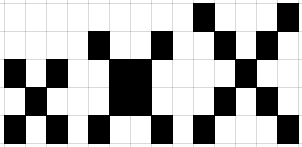
\includegraphics[scale=0.8]{modelo-x}
\centering
\caption{\enquote{X} em modelos de tamanhos diferentes}
\label{fig:xs}
\end{figure}

São apresentadas três versões desse modelo em ordem crescente de complexidade. O primeiro é um simples 3x3, o segundo possui dimensões 4x4 e o último modelo é uma grade 5x5. Cada um deles é representado computacionalmente por um vetor de zeros e uns.

O \enquote{X} na versão 3x3, por exemplo, é representado por [1, 0, 1, 0, 1, 0, 1, 0, 1]. Ou, em uma formatação que torna a visualização mais óbvia:

\begin{verbatim}
                             [1, 0, 1,
                              0, 1, 0,
                              1, 0, 1]
\end{verbatim}

Os vetores 3x3, 4x4 e 5x5 são representados respectivamente por:

\begin{verbatim}
              [1, 0, 1,     [1, 0, 0, 1,     [1, 0, 0, 0, 1,
               0, 1, 0,      0, 1, 1, 0,      0, 1, 0, 1, 0,
               1, 0, 1]      0, 1, 1, 0,      0, 0, 1, 0, 0,
                             1, 0, 0, 1]      0, 1, 0, 1, 0,
                                              1, 0, 0, 0, 1]
\end{verbatim}

A população é apresentada em três tamanhos: 10, 100 e 1000 indivíduos.

A probabilidade de mutação é apresentada em quatro configurações: 1/10, 1/100, 1/1000 e 0 (zero). A quarta configuração, 0 (zero), equivale efetivamente a remover o componente de mutação do algoritmo e acaba funcionando como um balisador para a relevância da mutação na solução.

Um dos problemas ao se remover a mutação do algoritmo é que a população inicial precisa possuir todos os \enquote{genes} suficientes para a resolução ou ele não chegará a uma solução. Por exemplo, considerando qualquer um dos modelos \enquote{X}, se na população inicial não houver sequer um indivíduo com o valor \enquote{1} na primeira posição do vetor, o algoritmo será incapaz de chegar à solução.

Cada um desses modelos é \enquote{resolvido} mil vezes e o número de gerações até a solução ser encontrada em cada uma delas é coletada para análise.

Como são 3 modelos, 3 tamanhos de população e 4 probabilidades de mutação, temos 36 experimentos ao total.

%
\subsection{Probabilidade de Cruzamento}
%
No algoritmo adotado não há \emph{probabilidade de cruzamento}. Uma vez que dois indivíduos são selecionados para cruzamento, eles sempre gerarão filhos e nunca serão transferidos para a geração seguinte.

Essa decisão simplifica o problema, diminuindo em um o número de parâmetros a ser analisado. Por outro lado, os melhores indivíduos têm boas chances de passar para a geração seguinte dependendo do tamanho da população, pois se selecionados pais iguais, filhos iguais serão gerados, efetivamente \enquote{preservando} o indivíduo de uma geração para seguinte.

É possível calcular essa probabilidade da sequinte forma:

\begin{align*}
P(\textnormal{preservação}) = 1 - \left(1 - P(\textnormal{escolha})^2\right)^{\textnormal{cruzamentos}}
\end{align*}

Sendo $P(\textnormal{escolha})$ a probabilidade de um indivíduo ser escolhido para cruzamento e \emph{cruzamentos} o número de cruzamentos a serem feitos para preservar o tamanho da população. Por exemplo, em uma população de 10 indivíduos e considerando que cada cruzamento gere 2 filhos, são necessários 5 cruzamentos para se preservar o tamanho da população. Nesse cenário, um indivíduo que tenha 10\% de chance de ser selecionado para cruzamento possui $1 - \left(1 - 0,1^2\right)^5 = 0,0602$, ou seja, cerca de 6\% de chance de ser preservado na geração futura. Nas mesmas condições, mas considerando uma população de 100 indivíduos a probabilidade de preservação sobe para aproximadamente 39,5\% e em 1.000 indivíduos fica em torno de 99,34\%.
%
\subsection{Tamanho do Espaço de Busca}
%
Um item importante a ser medido para se compreender o comportamento dos parâmetros é o tamanho do espaço de busca, no caso presente isso significa quantas configurações de zeros e uns são possíveis para cada tamanho do vetor.

A representação do indíduo como um vetor binário torna essa análise bastante simples. O tamanho do espaço de busca é dado por $2^{\textnormal{tamanho do vetor}}$. O número de elementos no vetor, por sua vez, é dado pela multiplicação dos lados da grade, ou seja, na grade 3x3 ele é 9, enquanto que na grade 5x5 possui tamanho 25. Em grades quadradas isso significa que o número de elementos de vetor é dado por $\textit{lado da grade}^2$.

A fórmula final para o tamanho do espaço de busca $s$ dado por:

\begin{align*}
\textnormal{tamanho do espaço de busca} = 2^{\textnormal{lado da grade}^2}
\end{align*}

Dessa forma, o tamanho dos espaços de busca para cada modelo são:

\begin{itemize}
\item 3x3: $2^{3^2} = 512$
\item 4x4: $2^{4^2} = 65.536$
\item 5x5: $2^{5^2} = 33.554.432$
\end{itemize}

Em outras palavras o espaço de busca cresce de maneira exponencial quadrática pelo tamanho da grade dos modelos apresentados.

%
\subsection{Probabilidade de Sucesso por Seleção Aleatória}
%
Uma medida útil para se compreender a eficiência do algoritmo genético é compará-lo com a probabilidade de se encontrar a solução para o problema ao se criar aleatoriamente um indivíduo.

A probabilidade de se encontrar o modelo ao se gerar um único indivíduo é de:

\begin{align*}
P(\textnormal{modelo}) = \frac{1}{\textnormal{tamanho do espaço de busca}}
\end{align*}

No caso do modelo 3x3, isso significa que $P(\textnormal{modelo 3x3}) = \frac{1}{512}$, enquanto que o modelo 5x5 diminui a probabilidade para $P(\textnormal{modelo 5x5}) = \frac{1}{33.554.432}$.

A criação de novos indivíduos aleatórios sucessivamente aumenta a probabilidade do modelo estar entre eles.

\begin{align*}
P(\textnormal{modelo}) = 1 - \left(\frac{\textnormal{tamanho do espaço de busca} - 1}{\textnormal{tamanho do espaço de busca} }\right)^{\textnormal{}} 
\end{align*}

Por exemplo, usando a grade 3x3, em 10 indivíduos aleatoriamente gerados como população inicial, existe a probabilidade de 1,93\% do modelo estar presente nessa população. Ao se gerar uma população de 1.000 indivíduos essa chance sobe para 85,84\%.

A probabilidade da solução ser encontrada aleatoriamente serve como base comparativa do algoritmo ou de seus parâmetros. Se as probabilidades forem similares, o algoritmo não é muito mais eficiente que uma busca aleatória, por outro lado, quanto maior a diferença entre as probabilidades, melhor é o desempenho do algoritmo.

Essa base nos permite comparar algoritmos com espaços de busca de tamanhos diferentes.

No caso do algoritmo genético, a execução de vários experimentos permite traçar uma distribuição aproximada de quantos indivíduos são necessários para alcançar a solução. Essa distribuição pode ser comparada à probabilidade de se encontrar a solução aleatoriamente para desenhar um quadro sobre o comportamento do sistema.

Para comparação, é preciso contabilizar o número de indivíduos gerados pelo algoritmo até a solução. A cada geração, ele cria uma nova população de igual tamanho a partir da população da geração anterior. Então, assumindo uma população de 1.000 indivíduos, a segunda geração terá criado outros 1.000 indivíduos, totalizando 2.000 indivíduos gerados no processo. O número de indivíduos gerados é simplesmente:

\begin{align*}
\textnormal{número de indivíduos criados} = \textnormal{população} \times \textnormal{número da geração}
\end{align*}

Assuma, para fins de ilustração, que no modelo 3x3 o algoritmo encontra a solução na 7ª geração \emph{em média}, precisando de 7.000 indivíduos para isso. Se fosse aplicado uma busca aleatória, a chance de se encontrar a solução com 7.000 indivíduos gerados é de cerca de 99,9998\%. Ou seja, em média o algoritmo não é muito diferente de se criar aleatoriamente indivíduos até esbarrar com a solução correta.

Na falta de um nome melhor, chamemos essa equivalência em probabilidade de \emph{índice de convergência}.

Gerando-se \emph{índices de convergência} para cada conjunto de parâmetros é possível compará-los diretamente \footnote{Ronie: me parece que estou no caminho certo de traçar uma equivalência entre uma busca aleatória e o algoritmo para poder compará-los com um único índice em espaços de busca diferentes, mas obviamente falta um último passo que não consegui chegar: "quão melhor isso é que uma busca aleatória?" :( Se conseguir chegar em um raciocínio para isso, acho que tem algo bem interessante que pode ser explorado na análise de outros algoritmos estocásticos. Por outro lado, não consegui achar na literatura algo nesse sentido, talvez eu não tenha usado os termos corretos (com certeza não li material suficiente para ver se não existe uma solução melhor na literatura)}.

%
\section{Resultados}
%
Os resultados dos experimentos se encontram na tabela 1. As três primeiras colunas mostram os parâmetros usados, as colunas seguintes mostram em que geração foi encontrada a solução.

O algoritmo restringe o número de gerações a 1.000, portanto, uma célula com esse valor significa que o algoritmo parou antes de conseguir chegar a uma solução.

Observa-se que os experimentos com apenas 10 individuos raramente chegam a encontrar uma solução nas 1.000 primeiras gerações, exceto para o problema mais simples de 3x3.

A quarta e quinta coluna mostram o intervalo de confiança de 95\% para se encontrar o modelo. Isso significa que em 95\% das vezes é possível encontrá-lo entre nesse intervalo de gerações. É possível observar que a variação diminui quando se aumenta a população, mas não parece sofrer grande influência da probabilidade de mutação.

As três colunas seguintes mostram o 1º, 2º (mediana) e 3º quartis. É possível observar que elas variam de acordo com o tamanho do espaço de busca, em menor grau pela população e quase não variam devido a probabilidade de mutação.

Finalmente, as últimas duas colunas mostram a quantidade média (mediana) de indivíduos necessária até se chegar ao modelo e a probabilidade dele ser encontrado se essa quantidade de indivíduos fosse aleatoriamente criada, o que chamamos anteriormente de \emph{Índice de Convergência}. Quanto menor essa porcentagem, mais longe o algoritmo está de desempenhar como uma mera busca aleatória.

É curioso observar que, nesses experimentos, um problema com espaço de busca reduzido não obtem grande benefício do uso de um Algoritmo Genético. Entretanto, conforme o espaço de busca aumenta, o algoritmo encontra a solução muito mais rapidamente em comparação com a busca aleatória.

Outro ponto a ser notado é que uma população reduzida não consegue gerar resultados no experimento, por outro lado, uma população muito grande tem um desempenho pior que a população de tamanho médio. Ao menos nesses experimentos, o tamanho \enquote{correto} da população para o tamanho do espaço de busca é o parâmetro mais relevante para a eficiência da solução.

Finalmente, nesse experimento, a probabilidade de mutação não modifica significativamente a busca. Como discutido anteriormente, dada uma população suficientemente grande para possuir todos os \enquote{genes} necessários para se chegar a uma solução, a mutação não seria estritamente necessária. No entanto, quanto mais \enquote{genes} forem precisos para se codificar o problema, mais difícil é para que a população inicial possuí-los todos.

\begin{table}
\centering
\begin{tabular}{|c|S|c|c|c|c|c|c|c|c|}
\hline
\multicolumn{3}{|c|}{Parâmetros} & \multicolumn{5}{|c|}{Geração até chegar à solução} & \multicolumn{2}{|c|}{Desempenho} \\ 
\hline
Grade & Mutação & População & \multicolumn{2}{|c|}{95\% de confiança} & 1º Quartil & Mediana & 3º Quartil & Indivíduos & IC \\ 
\hline
3x3 & 0.1 & 10 & 2 & 1000 & 16 & 167 & 435 & 1670 & 96,17\%\\ 
\hline
3x3 & 0.01 & 10 & 1 & 1000 & 12 & 132 & 383 & 1320 & 92,42\%\\ 
\hline
3x3 & 0.001 & 10 & 2 & 1000 & 40 & 197 & 430 & 1970 & 97,87\%\\ 
\hline
3x3 & 0 & 10 & 2 & 1000 & 32 & 135 & 404 & 1350 & 92,85\%\\ 
\hline
3x3 & 0.1 & 100 & 1 & 6 & 2 & 3 & 4 & 300 & 44,37\%\\ 
\hline
3x3 & 0.01 & 100 & 1 & 7 & 2 & 3 & 4 & 300 & 44,37\%\\ 
\hline
3x3 & 0.001 & 100 & 1 & 7 & 2 & 3 & 4 & 300 & 44,37\%\\ 
\hline
3x3 & 0 & 100 & 1 & 8 & 2 & 3 & 4 & 300 & 44,37\%\\ 
\hline
3x3 & 0.1 & 1000 & 1 & 2 & 1 & 1 & 1 & 1000 & 85,84\%\\ 
\hline
3x3 & 0.01 & 1000 & 1 & 2 & 1 & 1 & 1 & 1000 & 85,84\%\\ 
\hline
3x3 & 0.001 & 1000 & 1 & 2 & 1 & 1 & 1 & 1000 & 85,84\%\\ 
\hline
3x3 & 0 & 1000 & 1 & 3 & 1 & 1 & 1 & 1000 & 85,84\%\\ 
\hline
4x4 & 0.1 & 10 & 406 & 1000 & 1000 & 1000 & 1000 & 10000 & \\ 
\hline
4x4 & 0.01 & 10 & 535 & 1000 & 1000 & 1000 & 1000 & 10000 & \\ 
\hline
4x4 & 0.001 & 10 & 241 & 1000 & 1000 & 1000 & 1000 & 10000 & \\ 
\hline
4x4 & 0 & 10 & 185 & 1000 & 1000 & 1000 & 1000 & 10000 & \\ 
\hline
4x4 & 0.1 & 100 & 5 & 27 & 11 & 14 & 17 & 1400 & 2,11\%\\ 
\hline
4x4 & 0.01 & 100 & 5 & 38 & 11 & 14 & 16 & 1400 & 2,11\%\\ 
\hline
4x4 & 0.001 & 100 & 4 & 27 & 10 & 13 & 17 & 1300 & 1,96\%\\ 
\hline
4x4 & 0 & 100 & 6 & 26 & 11 & 14 & 18 & 1400 & 2,11\%\\ 
\hline
4x4 & 0.1 & 1000 & 2 & 10 & 5 & 7 & 8 & 7000 & 10,13\%\\ 
\hline
4x4 & 0.01 & 1000 & 2 & 11 & 5 & 7 & 8 & 7000 & 10,13\%\\ 
\hline
4x4 & 0.001 & 1000 & 3 & 10 & 5 & 7 & 8 & 7000 & 10,13\%\\ 
\hline
4x4 & 0 & 1000 & 2 & 10 & 5 & 7 & 8 & 7000 & 10,13\%\\ 
\hline
5x5 & 0.1 & 10 & 1000 & 1000 & 1000 & 1000 & 1000 & 10000 & \\ 
\hline
5x5 & 0.01 & 10 & 1000 & 1000 & 1000 & 1000 & 1000 & 10000 & \\ 
\hline
5x5 & 0.001 & 10 & 1000 & 1000 & 1000 & 1000 & 1000 & 10000 & \\ 
\hline
5x5 & 0 & 10 & 1000 & 1000 & 1000 & 1000 & 1000 & 10000 & \\ 
\hline
5x5 & 0.1 & 100 & 16 & 183 & 27 & 38 & 57 & 3800 & 0,011\%\\ 
\hline
5x5 & 0.01 & 100 & 18 & 257 & 30 & 41 & 53 & 4100 & 0,012\%\\ 
\hline
5x5 & 0.001 & 100 & 18 & 178 & 31 & 39 & 49 & 3900 & 0,011\%\\ 
\hline
5x5 & 0 & 100 & 17 & 178 & 29 & 37 & 50 & 3700 & 0,011\%\\ 
\hline
5x5 & 0.1 & 1000 & 10 & 25 & 16 & 19 & 22 & 19000 & 0,056\%\\ 
\hline
5x5 & 0.01 & 1000 & 12 & 25 & 16 & 19 & 21 & 19000 & 0,056\%\\ 
\hline
5x5 & 0.001 & 1000 & 11 & 25 & 17 & 19 & 21 & 19000 & 0,056\%\\ 
\hline
5x5 & 0 & 1000 & 11 & 24 & 16 & 18 & 21 & 18000 & 0,053\%\\ 
\hline
\hline\end{tabular}
\label{tab:resultados}
\caption{\small{Resultados brutos}} 
\end{table}

%
\section{Conclusões}
%
O experimento é pequeno para mostrar dados conclusivos, mas mostra indícios do comportamento dos parâmetros de maneira bastante consistente. Obviamente, alterações no algoritmo ou alterações na forma como o problema é representado devem alterar esse comportamento.

Futuros trabalhos podem ser feitos usando-se uma metodologia parecida, mas com modificações no algoritmo e no problema para validar os dados aqui obtidos.

%
% ---- Bibliography ----
%
\begin{thebibliography}{5}
%

\bibitem {castro}
de Castro, L.N.: Fundamentals of Natural Computing: Basic Concepts, Algorithms, and Applications. CRC Press (2006).

\bibitem{racket}
Felleisen, M., Findler, R.B., Flatt, M.: The Racket Manifesto. LIPIcs-Leibniz. (2015).

\bibitem{deb:agra}
Deb, K., Agrawal, S.: Understanding interactions among genetic algorithm parameters. Foundations of Genetic Algorithms. (1999).

\end{thebibliography}

\section*{Apêndice}

\subsection*{Código Fonte do Algoritmo}

\begin{lstlisting}
#lang racket/base
(require threading)
(require racket/list)

(provide individual
         individual-geno
         individual-fit
         result
         result-epochs
         result-best
         random-individual
         create-individual
         run-genetic
         run-genetic-with-seed)

; === Parameterization
; Model to fit
(define reference (make-parameter '(0 1 0 0 1 0 0 1 0)))
(define reference-size (make-parameter (length (reference))))
(define mutation-probability (make-parameter 0.01))

(struct result (epochs best) #:transparent)

(struct individual (geno fit) #:transparent)

(define (random-individual)
  (create-individual (random-genotype)))

(define (create-individual genotype)
  (individual genotype (fitness genotype)))

; Creates a random genotype
(define (random-genotype)
  (build-list (reference-size) (lambda (_x) (random 2))))

(define (create-population n)
  (build-list n (lambda (_x) (random-individual))))

(define (fitness genotype)
  (for/sum ([allel-r (reference)]
            [allel-g genotype])
    (if (= allel-g allel-r) 1 0)))

(define (similarity ind1 ind2)
  (define g1 (individual-geno ind1))
  (define g2 (individual-geno ind2))
  (define size (length g1))
  (define similar (for/sum ([a1 g1] [a2 g2])
                    (if (= a1 a2) 1 0)))
  (/ similar size))

(define (wheel-for population)
  (for/fold ([rslt empty])
            ([ind population])
    (let* ([fit (individual-fit ind)]
           [fitness-list (make-list fit ind)])
      (append rslt fitness-list))))

(define (wheel->picker wheel)
  (define wheel-length (length wheel))
  (lambda () (~>> wheel-length random (list-ref wheel))))

(define (generate-picker population)
  (~> (wheel-for population) wheel->picker))

(define (crossover . parents)
  (define point (random (reference-size)))
  (define genotypes (map individual-geno parents))
  (define-values (g11 g12) (split-at (first genotypes) point))
  (define-values (g21 g22) (split-at (second genotypes) point))
  (map create-individual (list (append g11 g22) (append g21 g12))))

(define (mutate ind [probability (mutation-probability)])
  (define point (random (reference-size)))
  (define genotype (individual-geno ind))
  (define (change allel) (if (= 1 allel) 0 1))
  (define new-geno (for/list ([(x i) (in-indexed genotype)])
                     (if (and (< (random) probability)
                              (= i point))
                        (change x) x)))
  (create-individual new-geno))

(define (breed p1 p2)
  (define sons (crossover p1 p2))
  (map mutate sons))

(define (run-genetic model target-fitness
                     #:population [initial-population 25]
                     #:limit [epoch-limit 1000]
                     #:mutation [mutation 0.01])
  (parameterize ([reference model]
                 [reference-size (length model)]
                 [mutation-probability mutation])
    (run-genetic-with-seed model target-fitness
                           (create-population initial-population)
                           #:limit epoch-limit)))

(define (run-genetic-with-seed model target-fitness initial-population
                               #:limit [epoch-limit 1000]
                               #:mutation [mutation 0.01])
  (parameterize ([reference model]
                 [reference-size (length model)]
                 [mutation-probability mutation])
    (define (epoch-for population [epoch 1])
      (define best-elems (sort population > #:key individual-fit))
      (define best (first best-elems))
      (cond
        [(>= epoch epoch-limit) (result epoch best)]
        [(>= (individual-fit best) target-fitness) (result epoch best)]
        [else (epoch-for (new-generation population) (add1 epoch))]))
    (define (new-generation population)
      (define picker (generate-picker population))
      (let loop ([rslt '()])
        (if (>= (length rslt) (length initial-population))
            rslt
            (loop (append rslt (breed (picker) (picker)))))))
    (epoch-for initial-population)))
\end{lstlisting}

\subsection*{Código Fonte do Experimento}

\begin{lstlisting}
#lang racket/base
(require "genetic-algorithm.rkt")
(require racket/format)
(require math)

(define model-3x3 '(1 0 1
                    0 1 0
                    1 0 1))

(define model-4x4 '(1 0 0 1
                    0 1 1 0
                    0 1 1 0
                    1 0 0 1))

(define model-5x5 '(1 0 0 0 1
                    0 1 0 1 0
                    0 0 1 0 0
                    0 1 0 1 0
                    1 0 0 0 1))

(define pops '(10 100 1000))
(define muts '(0.1 0.01 0.001 0.0))

(define (run-experiment model population mut)
  (build-list 1000 (lambda (_x) (run-genetic model
                                        (length model)
                                        #:population population
                                        #:mutation mut))))

(for* ([name+model (list (cons "3x3" model-3x3)
                         (cons "4x4" model-4x4)
                         (cons "5x5" model-5x5))]
       [population pops]
       [mutation-rate muts])
  (let* ([rslt (run-experiment (cdr name+model) population mutation-rate)]
         [generations (map result-epochs rslt)])
    (printf "===== ~a\n" (car name+model))
    (printf " Mutation rate: ~a\n" (~r mutation-rate #:precision 3))
    (printf "    Population: ~a\n" population)
    (printf "Confidence 95%: ~a to ~a\n"
            (quantile 0.025 < generations)
            (quantile 0.975 < generations))
    (printf "  1st Quartile: ~a\n" (quantile 1/4 < generations))
    (printf "        Median: ~a\n" (quantile 2/4 < generations))
    (printf "  3rd Quartile: ~a\n" (quantile 3/4 < generations))
    (flush-output)))
\end{lstlisting}

\end{document}
